\documentclass[tikz,border=5mm, 11pt]{standalone}

\usepackage{pgfplots}
\usepackage{amsmath}
\usepackage{amssymb}
\pgfplotsset{compat=1.18}

\usepackage[no-math]{fontspec}
\usepackage{unicode-math}
%\setmainfont{Lato}
%\setmathfont{Stix Two Math}
\usepackage{mlmodern}
\usepackage[sfdefault, scaled=0.9]{inter}
\usepackage{siunitx}

\usepackage{pgf,xcolor}
\definecolor{itwm_blue_04}{HTML}{005A94}
\definecolor{itwm_red}{HTML}{C00000}
\definecolor{itwm_yellow}{HTML}{FFEC7F}
\definecolor{mygrey}{HTML}{484949}

\usepackage{tikz}
\usetikzlibrary{shapes.misc, shadows, decorations, arrows}
\usetikzlibrary{backgrounds}
\usetikzlibrary{calc}
\usepackage{pgfplots}
\pgfplotsset{compat=newest}
\usepgfplotslibrary{fillbetween}
\usepackage{tikzpagenodes}
\usetikzlibrary{patterns}

% 0,1 x 1,2
\begin{document}
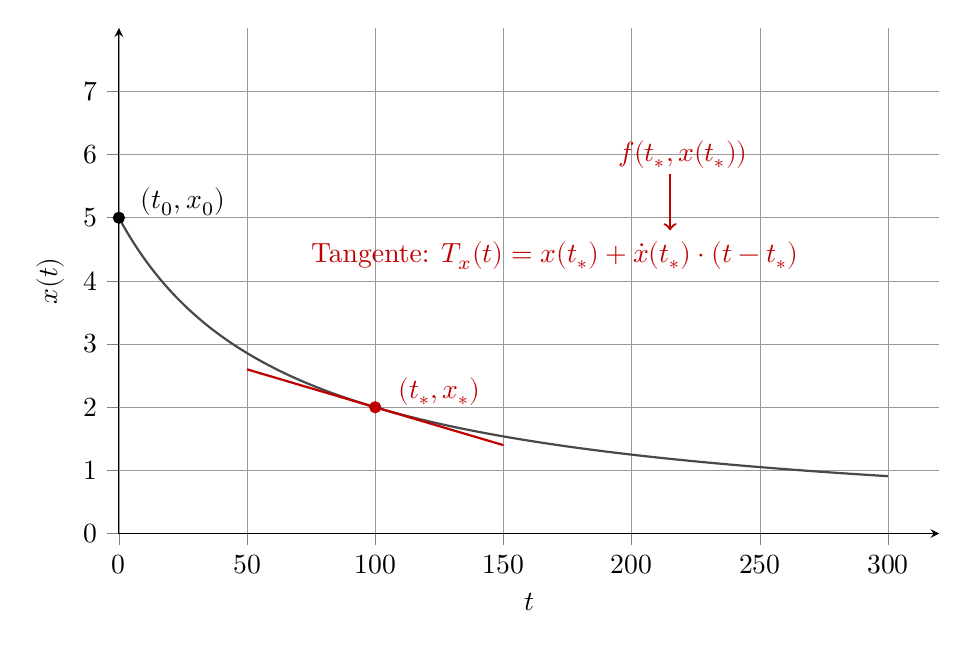
\begin{tikzpicture}
\begin{axis}[
    width=12cm,
    height=8cm,
    xlabel={$t$},
    ylabel={$x(t)$},
    %title={Anfangswertproblem $\dot{x}(t) = f(t, x(t)), \quad x(t_0) = x_0$},
    grid=major,
    grid style={line width=.1pt, draw=gray!50},
    major grid style={line width=.2pt, draw=gray!80},
    xmin=0, xmax=320,
    ymin=0, ymax=8,
    xtick={0, 50,100,150,200,250,300},
    ytick={0,1,2,3,4,5, 6, 7},
    axis lines=left,
    tick align=outside,
    legend pos=north east,
    samples=300,
    smooth,
]

% Plot der Funktion
\addplot[
    domain=0:300,
    mygrey,
    thick,
    samples=300
] {5/(0.015*x + 1)};

% Markierung einiger wichtiger Punkte
\addplot[only marks, mark=*, mark size=2pt] coordinates {
    (0, 5)
};
\node at (axis cs:0+25,5+0.25) {$(t_0,x_0)$};
\addplot[only marks, mark=*, mark size=2pt, itwm_red] coordinates {
    (100, 2)
};
\node[itwm_red] at (axis cs:100+25,2+0.25) {$(t_{*},x_{*})$};

% Beschriftung mit Pfeil für f(t, x(t))
\node[itwm_red] at (axis cs:220,6.0) {$f(t_{*}, x(t_{*}))$};
\draw[->, thick, itwm_red] (axis cs:215,5.7) -- (axis cs:215,4.8);

% Plot der Tangente
\addplot[
	domain=50:150,
	itwm_red,
	thick,
	samples=300
] {-0.012*x+3.2};
\node[itwm_red] at (axis cs:170,4.4) {Tangente: $T_{x}(t) = x(t_{*}) + \dot{x}(t_{*})\cdot(t-t_{*})$};
\end{axis}
\end{tikzpicture}

\end{document}
